\input{commun/presentations.tex}
\input{commun/video.tex}
\def\siecle#1{\textsc{\romannumeral #1}\textsuperscript{e}~siècle}

\title[Séance 12 - Vol stabilisé]{Séance 12 \\ Étude du vol stabilisé}

\begin{document}
 \begin{frame}
 \titlepage
 \end{frame}
 
 \begin{frame}{Introduction}
 	Les événements présentés ici sont une sélection des événements à connaitre pour l'examen, afin de donner les grandes lignes.
 	
 	Une frise plus complète est disponible en ligne : https://brevet.initiation.aero/friseChronologique.html
 \end{frame}
 
 \begin{frame}
 \tableofcontents
 \end{frame}
 
 \section{Le vol stabilisé}
 	\begin{frame}{Le vol stabilisé : définition}
 	Le vol est dit stabilisé quand les paramètres de vitesse (horizontale \& verticale) sont stables. \newline
 	
 	 L'aéronef suit alors un mouvement rectiligne uniforme (la trajectoire est une droite et la vitesse est constante). \newline
 	 
 	 Note : par simplification, on considérera pour cette séance que le poids et la portance s'appliquent au centre de gravité.
 	
 	\end{frame}
 	
 	\subsection{Vol stabilisé en palier}
 	\begin{frame}{Vol stabilisé en palier}
 	\begin{figure}[H]
			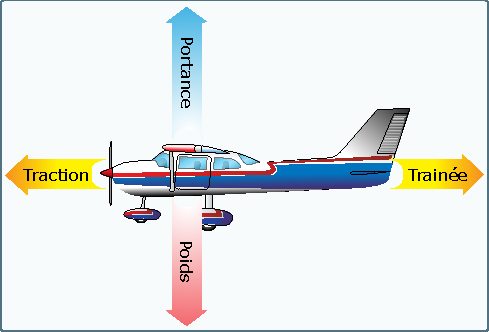
\includegraphics[width=0.7\linewidth]{04-Aerodynamique/img/forces}
			\legende{Les forces sur un aéronef en vol stabilisé en palier}{img:forces}
		\end{figure}	
 	
 	\end{frame}
 	
	
	\subsection{Vol stabilisé en montée ou descente}
	\begin{frame}{Vol stabilisé en montée}
	\begin{columns}
		\begin{column}{0.4\textwidth}
		\begin{figure}[H]
			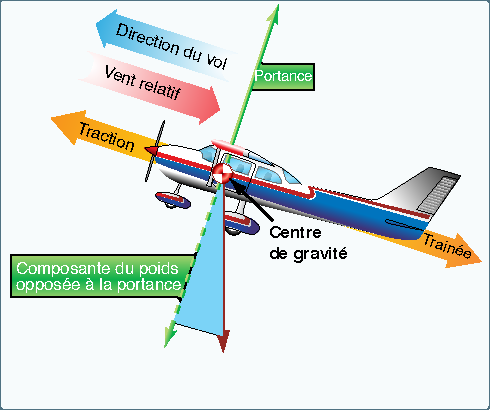
\includegraphics[width=1\linewidth]{04-Aerodynamique/img/forcesMontee}
			\legende{Forces s'appliquant sur un vol stabilisé en montée}{img:forcesMontee}
		\end{figure}	
		\end{column}
		\begin{column}{0.6\textwidth}
			
		\end{column}
		\end{columns}

	\end{frame}
	
	\section{Le facteur de charge}
	\begin{frame}{Le facteur de charge}
	\begin{columns}
		\begin{column}{0.4\textwidth}
		\begin{figure}[H]
			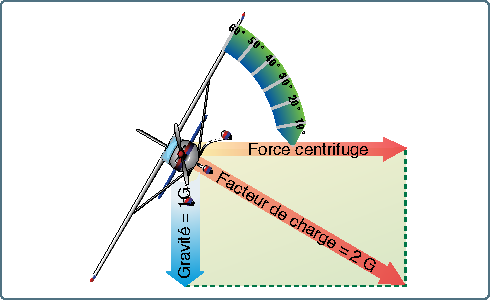
\includegraphics[width=1\linewidth]{04-Aerodynamique/img/virage60degres}
			\legende{Facteur de charge à 60\degree}{img:virage60degres}
		\end{figure}	
		\end{column}
		\begin{column}{0.6\textwidth}
			Quand un aéronef effectue un virage, il est soumis une accélération : le facteur de charge.
			
			Le facteur de charge est directement fonction de l'inclinaison, selon la formule $\dfrac{1}{cos(inclinaison)}$. \newline \pause
			
			Par conséquence, pour conserver le palier en virage, le pilote doit augmenter la portance par augmentation de la vitesse ou de l'incidence.
		
		\end{column}
		\end{columns}
		
	\begin{table}[]
\begin{tabular}{|l|l|l|l|l|}
\hline
Inclinaison (\degree) & 0 & 30   & 45   & 60 \\
\hline
Facteur de charge (G)                & 1 & 1,15 & 1,41 & 2 \\
\hline
\end{tabular}
\end{table}
	\end{frame}
	
	\begin{frame}{Le facteur de charge}
	\begin{columns}
		\begin{column}{0.4\textwidth}
		\begin{figure}[H]
			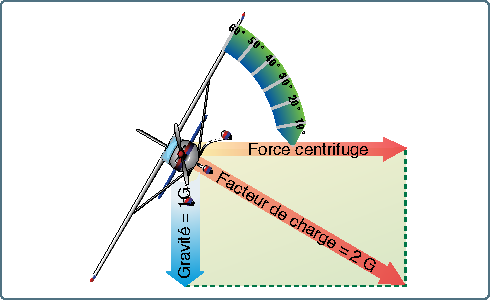
\includegraphics[width=1\linewidth]{04-Aerodynamique/img/virage60degres}
			\legende{Facteur de charge à 60\degree}{img:virage60degres}
		\end{figure}	
		\end{column}
		\begin{column}{0.6\textwidth}
			Rappel : l'augmentation de la portance augmente également la trainée. Toute mise en virage sans augmentation de la traction provoquera donc une baisse de la vitesse, qui nécessitera elle même une augmentation de l'incidence pour conserver la portance.
			
			Pour cette raison, a basse vitesse, on réalise de préférence des virages à \textbf{vitesse constante} : on augmente la puissance en début de virage pour empêcher la diminution de la vitesse.
		\end{column}
		\end{columns}
		
		En montée, on aura une vitesse faible et on sera généralement à pleine puissance. On limite donc l'inclinaison (généralement 20\degree) pour éviter d'approcher de l'incidence de décrochage.

	\end{frame}
	
	
\appendix 

\section{Consignes pour l'examen}
\begin{frame}{Mercredi 20 mai 2026 : BIA}
\begin{itemize}
	\item L'examen aura lieu au collège
	\item Répondre à toutes les questions :
	\begin{itemize}
		\item pas de point retiré en cas de mauvaise réponse
		\item en cas de doute sur une question, laissez la de côté et revenez y plus tard
	\end{itemize}
	\item N'hésitez pas à utiliser le brouillon à votre disposition, à entourer/barrer des réponses sur le sujet
	\item 20 questions sur les 5 thèmes (2h30) + épreuve d'anglais (30 minutes)
	\begin{itemize}
		\item météorologie et aérologie
		\item aérodynamique, aérostatique et principes du vol
		\item étude des aéronefs et des engins spatiaux
		\item navigation, réglementation, sécurité des vols
		\item histoire et culture de l'aéronautique et du spatial
		\item anglais
	\end{itemize}
\end{itemize}

\end{frame}

\section{QCM}
\qmcBia{Aérodynamique, aérostatique et principes du vol}
{2}{Pour un aéronef en montée rectiligne uniforme, la force de traction de l'hélice est fonction :}
{uniquement de la traînée}
{de la traînée, du poids et de l'angle de montée}
{uniquement du poids et de la portance}
{du poids et de l'angle de montée} 
{}

\qmcBia{Aérodynamique, aérostatique et principes du vol}
{3}{En vol, le facteur de charge d'un avion :}
{ne dépend que du poids de l'équipage et des bagages embarqués dans l'avion}
{est supérieur à 1 quand l'avion est en montée}
{augmente la vitesse de décrochage quand le facteur de charge augmente}
{est le rapport entre la masse et la surface des ailes de l'avion} 
{}


 
\input{commun/beamerSlidesBiblio.tex} 
 
\end{document}
